Equilateral triangle $ T$ is inscribed in circle $ A$, which has radius $ 10$. Circle $ B$ with radius $ 3$ is internally tangent to circle $ A$ at one vertex of $ T$. Circles $ C$ and $ D$, both with radius $ 2$, are internally tangent to circle $ A$ at the other two vertices of $ T$. Circles $ B$, $ C$, and $ D$ are all externally tangent to circle $ E$, which has radius $ \frac {m}{n}$, where $ m$ and $ n$ are relatively prime positive integers. Find $ m + n$.
\begin{center}
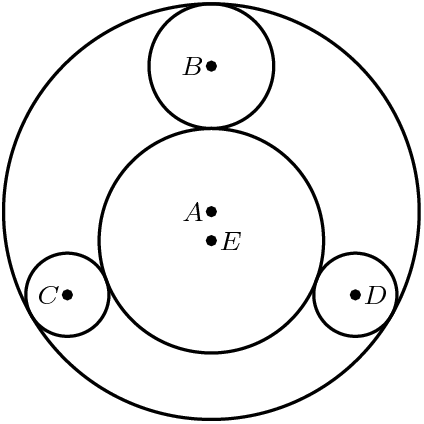
\includegraphics[width = 42.400000000000006mm]{img/fig0.png}
\end{center}